\documentclass[12pt,a4paper]{report}
% \textheight = 30cm
% \voffset = -36pt
\footskip = 0cm

\usepackage{cmap}
\usepackage{type1ec}
\usepackage[T2A]{fontenc}
\usepackage[utf8]{inputenc}
\usepackage[russian]{babel}

\usepackage{amsmath,amstext,amssymb}
\usepackage{fullpage}

\usepackage{ifpdf}
\ifpdf
  \usepackage[pdftex]{graphicx}
  \usepackage[pdftex,unicode,bookmarks=false]{hyperref}

  \pdfminorversion=5
  \pdfcompresslevel=9
  \pdfobjcompresslevel=9
\fi

\pagestyle{empty}

\graphicspath{{./figures/}}

\DeclareMathOperator{\EX}{\mathbb{E}}

\renewcommand{\thesection}{\arabic{section}}
\renewcommand{\thesubsection}{}

% Модуль
\providecommand{\abs}[1]{\left\lvert{#1}\right\rvert}

\begin{document}

% --------------------------------------------------------------------------------------

\section{Administrivia}

В прошлом году лекции и семинары практически не отличались, в этом попробуем решать больше задач на семинарах.

\subsection*{Оценка}

$$
G_{final} = 0.3 \cdot G_{hw} + 0.3 \cdot G_{test} + 0.4 \cdot G_{exam}
$$

Домашние задания -- после семинаров. Контрольная -- между модулями.

\subsection*{План}

1-й модуль:

\begin{itemize}
	\item Анализ сложности алгоритмов
	\item Алгоритмы сортировки
	\item Структуры данных: списки, деревья, хэш-таблицы, кучи, системы непересекающихся множеств
\end{itemize}

2-й модуль:

\begin{itemize}
	\item Жадное программирование. Динамическое программирование.
	\item Алгоритмы на графах.
	\item Алгоритмы на строках.
	\item Что-нибудь специфичное для лингвистики/численных методов/баз данных
\end{itemize}

\subsection*{Литература}

\begin{enumerate}
  \item {\bf T.~Cormen et al. {\em Introduction to Algorithms}}
  \item Steven Skiena {\em The Algorithm Design Manual}
  \item Бабенко М.А.,~Левин М.В. {\em Введение в теорию алгоритмов и структур данных}
\end{enumerate}

% --------------------------------------------------------------------------------------

\section{Алгоритмы}

{\em Алгоритм} -- в очень узком смысле -- спецификация решения задачи с помощью компьютера, подразумевающей преобразование входных данных в выходные. Строгость такой спецификации должна быть достаточной для создания компьютерной программы (реализации алгоритма), решающей эту задачу.

Подавляющая часть описываемых в курсе алгоритмов уже имеет свои реализации в стандартных и сторонних библиотеках языков программирования. Хотелось бы просто использовать их, не изучая стоящих за ними алгоритмов, но
\begin{itemize}
	\item абстракции протекают: эффективное использование библиотечных функций часто требует понимания работы и сложности реализованных алгоритмов (hashing trick, sparce matrix, graphs, индексы в базах данных, ...);
	\item иногда требуется реализовать новый алгоритм или структуру данных в условиях, с которыми ещё никто не сталкивался;
	\item подробнее -- в повести {\em Профессия} Айзека Азимова.
\end{itemize}

Термины и действия, в которых описывается алгоритм, зависят от выбранной модели вычислений.
Фактически -- некоторое абстрактное описание того, как именно работает компьютер, для которого предназначен алгоритм.

% --------------------------------------------------------------------------------------

\section{Word RAM model}

Модель аппроксимирует устройство всех современных компьютеров с достаточной для наших целей точностью.

\begin{itemize}
	\item Память: 
	\begin{itemize}
		\item Составлена из элементарных двоичных элементов памяти -- битов. Биты объединены в ячейки ({\em слова}) ширины $w$. Каждая ячейка имеет {\em адрес} -- число от $0$ до $M-1$.
		\item В реальных процессорах значений $w$ несколько -- 8/16/32/64 бит. Отсюда размеры числовых типов в языках программирования.
		\item {\em Байт}, по определению -- минимальная адресуемая ячейка памяти.
		\item Если нужно представить число большее чем $2^w-1$, используем несколько ячеек.
		\item {\em Массив} -- конечное число последовательно расположенных ячеек памяти
		\item {\em Строка} -- массив чисел, соответствующих буквам согласно кодировке (ASCII, UTF-8, ...)
	\end{itemize}
	\item CPU: 
	\begin{itemize}
		\item Фиксированное число {\em регистров} $\{r_i\}$ -- встроенных неадресуемых ячеек памяти размера $w$ каждая.
		\item Исполняет {\em программу} -- список пронумерованных операций:
		\begin{itemize}
			\item {\tt load RAM[rx] -> ry}\\
				  загрузить значение ячейки по адресу $r_x$ в регистр $r_y$
			\item {\tt store ry -> RAM[rx]}\\
			      записать значение из регистра $r_y$ в память по адресу $r_x$\\
			      кстати, отсюда же следует что $M \leq 2^w$
			\item {\tt add r1, r2 -> r3}\\
				  сложить числа в регистрах $r_1$ и $r_2$, записать результат в $r_3$
			\item {\tt sub r1, r2 -> r3}
			\item {\tt mul r1, r2 -> r3, r4}
			\item {\tt div r1, r2 -> r3, r4}
			\item {\em побитовые логические операции, сдвиги, операции над числами с плавающей точкой, и любые другие процессорозависимые операции, если мы хотим добавить их в модель}
			\item {\tt jcmp r1, r2 -> L}\\
				  переходит к операции под меткой $L$ если $r_1 < r_2$,
		\end{itemize}
		\item Каждая операция исполняются за единицу времени, т.е. их можно считать элементарными
		\item Программы на любых языках программирования в конце концов транслируются в элементарные операции.
	\end{itemize}
\end{itemize}

Условно, имея в виду эту модель и достаточно современные компьютеры, арифметические операции над целыми числами не превышающими $2^{64}-1$ можно считать выполняющимися за некоторое постоянное время $t_0$, при этом у разных компьютеров $t_0$ будет различным.


\section{Сложность алгоритма}

Цель: минимизировать потребление ресурсов алгоритмом. Ресурсы: время работы и потребляемая во время исполнения память.

Выразим время работы алгоритма как функцию от входных данных $I$ и $t_0$.
$$
T(I, t_0)
$$
-- это полноценная функция в математическом смысле: у детерменированного алгоритма для одних и тех же данных на одном компьютере время работы должно быть одинаковым.

Практичнее, однако, в качестве параметра использовать не сами данные, а их размер (количество элементов массива, размерность матрицы, количество вершин и рёбер графа, разрядность входного числа, и т.~п.)
$$
T'(n, t_0)
$$

Но $T'$ не является функцией. Например, сортировка массивов размера $n$ может сильно отличаться по времени, в зависимости от начального разположения элементов. Необходимо как-то аггрегировать все возможные данные размера $n$. Тут возможны варианты:
$$
T_w(n, t_0) = \max_{I \in I_n}~{T(I, t_0)}
$$
-- {\em сложность в худшем случае} ({\em worst-case complexity}).

$$
T_e(n, t_0) = \mathbb{E}_{I \in I_n} \left[ {T(I, t_0)} \right]
$$
-- {\em ожидаемая сложность}, или сложность в среднем, если брать равномерное распределение входных данных.

Теперь нужно избавиться от $t_0$: его значение практически невозможно посчитать на практике. Но кроме того, оно даёт лишь константный вклад во время работы алгоритма. Гораздо больше нас интересует то, как быстро растёт функция времени при увеличении $n$.


\section{Асимптотический анализ}

\begin{figure}
\centering
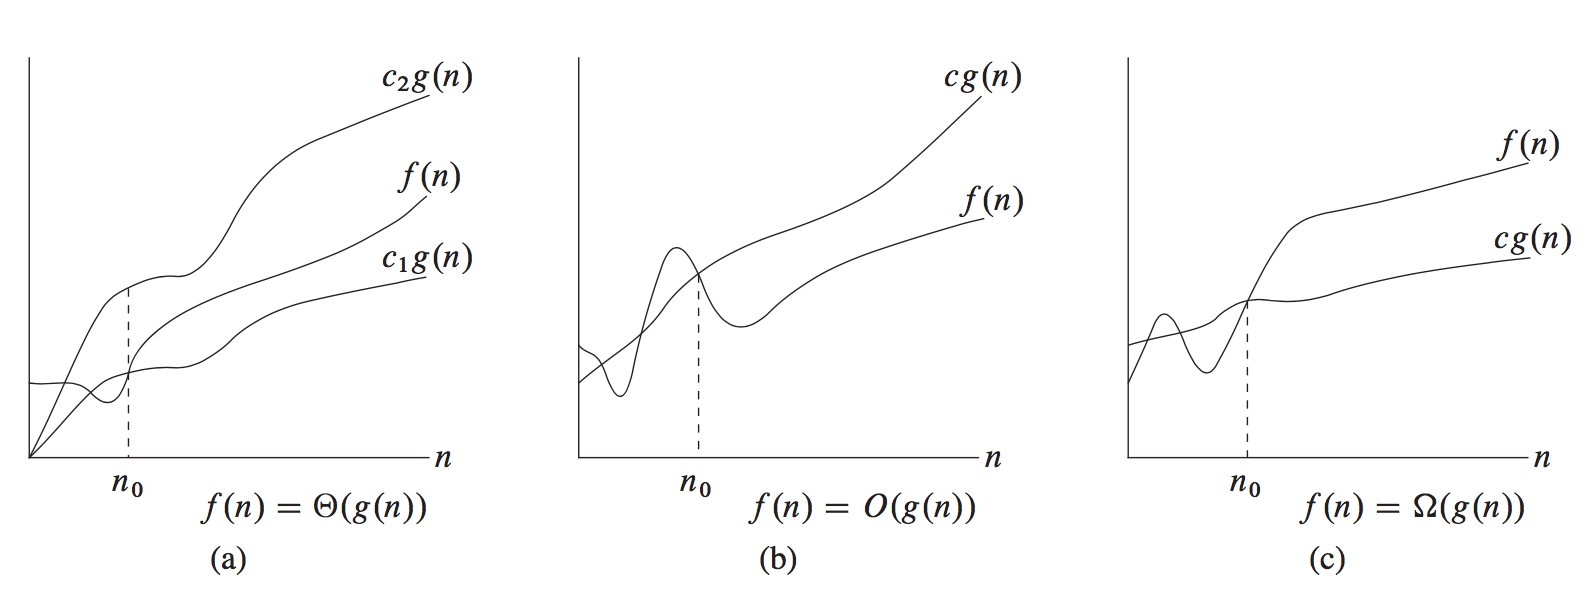
\includegraphics[width=11cm]{classes.png}
\end{figure}

Будет рассматривать функцию времени $T(n)$ при $n \to \infty$. Введём класс функций:

$$
\Theta(g(n)) = \{f(n) : \exists c_1, c_2, n_0: \forall n > n_0 ~\to~ 0 \leqslant c_1 \cdot g(n) \leqslant f(n) \leqslant c_2 \cdot g(n) \\
$$

Иначе говоря, $f(n)$ принадлежит классу $\Theta(g(n))$ если можно подобрать $c_1$ и $c_2$ так, что для достаточно больших $n$ функция оказывается <<зажатой>> между $c_1 \cdot g(n)$ и $c_2 \cdot g(n)$. Будет обозначать принадлежность к классу как $f(n) = \Theta(g(n))$.

Найдя для $f(n)$ подходящий класс $\Theta(g(n))$, можно будет сказать, что $f(n)$ и $g(n)$ отличается не более чем на константу. Важно, что при поиске подходящего класса можно игнорировать константы и члены низшего порядка в $f(n)$. Например:

$$
f(n) = an^2 + bn + c
$$

Докажем, что $f(n) = \Theta(n^2)$. Подставив в определение значения констант:
$$
c_1 = a/4 ~~~~ c_2 = 7a/4 ~~~~ n_0 = 2 \cdot \max\{\abs{b}/a, \sqrt{\abs{c}/a}\}
$$
можно проверить, что:
$$
\forall n > n_0 ~\to~ 0 \leqslant c_1 n^2 \leqslant an^2 + bn + c \leqslant c_2 n^2
$$

В общем случае можно доказать, что полином $p(n) = \sum_{i=0}^{d} a_i n^i = \Theta(n^d)$ при $a_d > 0$.

Можно также ввести отдельные классы, дающие соответственно верхнюю и нижнюю оценку функции:
$$
\begin{gathered}
O(g(n)) = \{f(n) : \exists c, n_0: \forall n > n_0 ~\to~ 0 \leqslant f(n) \leqslant c \cdot g(n) \\
\Omega(g(n)) = \{f(n) : \exists c, n_0: \forall n > n_0 ~\to~ 0 \leqslant c \cdot g(n) \leqslant f(n)
\end{gathered}
$$

Для $O$ или $\Omega$, согласно определениям, верны нестрогие оценки: $2n = O(n^2)$, $100n^3 = \Omega(n)$. Для таких оценок существуют отдельные классы, знакомые вам по курсу матанализа:

$$
\begin{gathered}
o(g(n)) = \{f(n) : \forall c ~ \exists n_0: \forall n > n_0 ~\to~ 0 \leqslant f(n) \leqslant c \cdot g(n) \\
\omega(g(n)) = \{f(n) : \forall c ~ \exists n_0: \forall n > n_0 ~\to~ 0 \leqslant c \cdot g(n) \leqslant f(n)
\end{gathered}
$$

Иначе говоря, $f(n)=o(g(n))$ означает, что $g(n)$ растёт быстрее $f(n)$ на бесконечности:
$$
f(n)=o(g(n))  ~~~\Leftrightarrow~~~ \lim_{n\to\infty} \frac{f(n)}{g(n)} = 0
$$

аналогично
$$
f(n)=\omega(g(n))  ~~~\Leftrightarrow~~~ \lim_{n\to\infty} \frac{f(n)}{g(n)} = \infty
$$

Принадлежность к $\Theta$ также удобно вычислять через предел:
$$
\begin{gathered}
\lim_{n\to\infty} \frac{f(n)}{g(n)} = C > 0   ~~~\Rightarrow~~~   f(n) = \Theta(g(n))
\end{gathered}
$$

\subsection*{Итог}

Время работы и потребление памяти не оценивается в абсолютных единицах, поскольку они могут варьироваться в зависимости от языка программирования, компьютера и многих деталей реализации. Вместо этого ресурсы оцениваются асимптотическими классами, которые можно сранивать не оглядываясь на конкретные реализации.

\section{Пример: сортировка вставками}

\begin{verbatim}
def insertion_sort(A):
    for j in range(1, len(A)):
        # В этой точке отсортированый префикс в массиве
        # имеет длину j
        key = A[j]
        i = j
        while i>0 and A[i-1]>key:
            A[i] = A[i-1]
            i -= 1
        A[i] = key
    return A
\end{verbatim}



\end{document}